\begin{pa} \label{PA:6.2}  Consider a circular cone of radius 3 and height 5, which we view horizontally as pictured in Figure~\ref{F:PA.6.2}.  Our goal in this activity is to use a definite integral to determine the volume of the cone.

\ba
	\item Find a formula for the linear function $y = f(x)$ that is pictured in Figure~\ref{F:PA.6.2}.
	\item For the representative slice of thickness $\triangle x$ that is located horizontally at a location $x$ (somewhere between $x = 0$ and $x = 5$), what is the radius of the representative slice?  Note that the radius depends on the value of $x$.
	\item What is the volume of the representative slice you found in (b)?
	\item What definite integral will sum the volumes of the thin slices across the full horizontal span of the cone?  What is the exact value of this definite integral?
	\item Compare the result of your work in (d) to the volume of the cone that comes from using the formula $V_{\text{\small{cone}}} = \frac{1}{3} \pi r^2 h.$
\ea

\begin{figure}[h]
\begin{center}
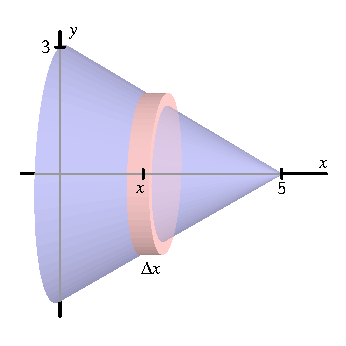
\includegraphics{figures/6_2_PA1.eps}
\caption{The circular cone described in Preview Activity~\ref{PA:6.2}} \label{F:PA.6.2}
\end{center}
\end{figure}

\end{pa} 
\afterpa